
\documentclass{beamer}

% This file is a solution template for:

% - Giving a talk on some subject.
% - The talk is between 15min and 45min long.
% - Style is ornate.



% Copyright 2004 by Till Tantau <tantau@users.sourceforge.net>.
%
% In principle, this file can be redistributed and/or modified under
% the terms of the GNU Public License, version 2.
%
% However, this file is supposed to be a template to be modified
% for your own needs. For this reason, if you use this file as a
% template and not specifically distribute it as part of a another
% package/program, I grant the extra permission to freely copy and
% modify this file as you see fit and even to delete this copyright
% notice. 


\mode<presentation>
{
  \usetheme{Warsaw}
  %\usetheme{Darmstadt}
  % or ...

  \setbeamercovered{transparent}
  % or whatever (possibly just delete it)
  \definecolor{burntorange}{RGB}{224,96,6}
  \definecolor{mdablue}{RGB}{127,199,206}
  \setbeamercolor{structure}{fg=mdablue}
  \usecolortheme{whale}
}

% define directories for movies and pics
\newcommand{\picdir}{pdffig}
\newcommand{\moviedir}{Movies}


\usepackage[english]{babel}
% or whatever

\usepackage[latin1]{inputenc}
% or whatever

\usepackage{times}
%\usepackage{animate}
%\usepackage{movie}
\usepackage[T1]{fontenc}
% Or whatever. Note that the encoding and the font should match. If T1
% does not look nice, try deleting the line with the fontenc.

\usepackage{boxedminipage}
\usepackage{multirow,float}

\graphicspath{{\picdir/}}
%\DeclareGraphicsRule{.pdftex}{pdf}{*}{}

\begin{document}
%%%%%%%%%%%%%%%%%%%%%%%%%%%%%%%%%%%%%%%%%%%%%%%%%%%%%%%%%%%%%%%%%%%%%%%%%%%
\frame{
\frametitle{B.B. software stack}
\framesubtitle{(Before BrainNek)}
\scalebox{0.36}{ 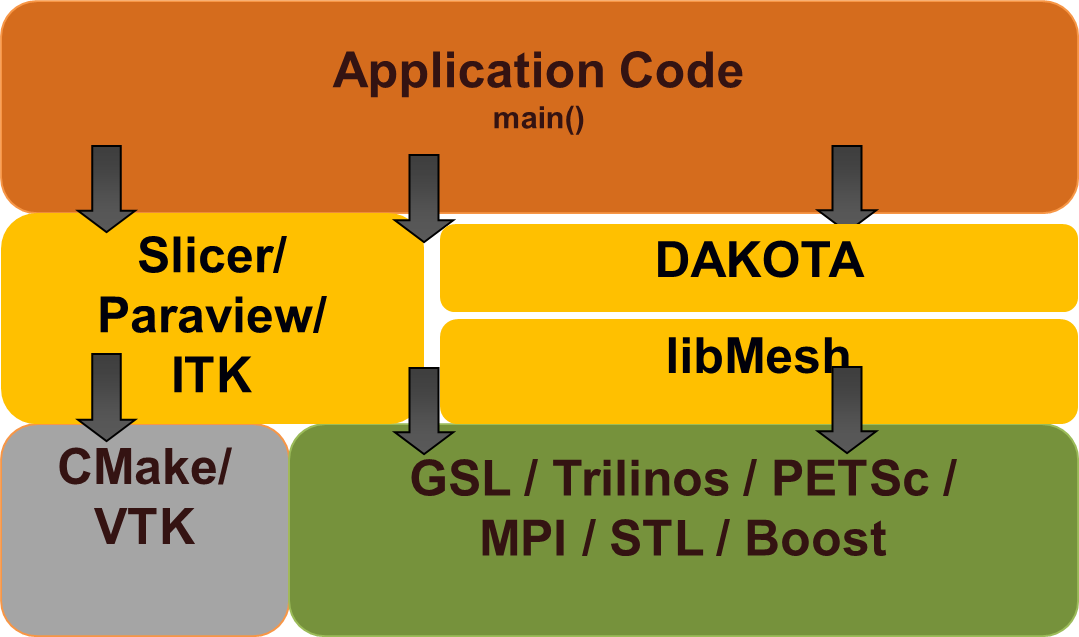
\includegraphics{\picdir/SoftwareStack}}
}
%%%%%%%%%%%%%%%%%%%%%%%%%%%%%%%%%%%%%%%%%%%%%%%%%%%%%%%%%%%%%%%%%%%%%%%%%%%
\begin{frame}
\frametitle{B.B software stack}
Remote vis needed to access and visualize simulation results on 
large super computing clusters.
\scalebox{0.36}{ 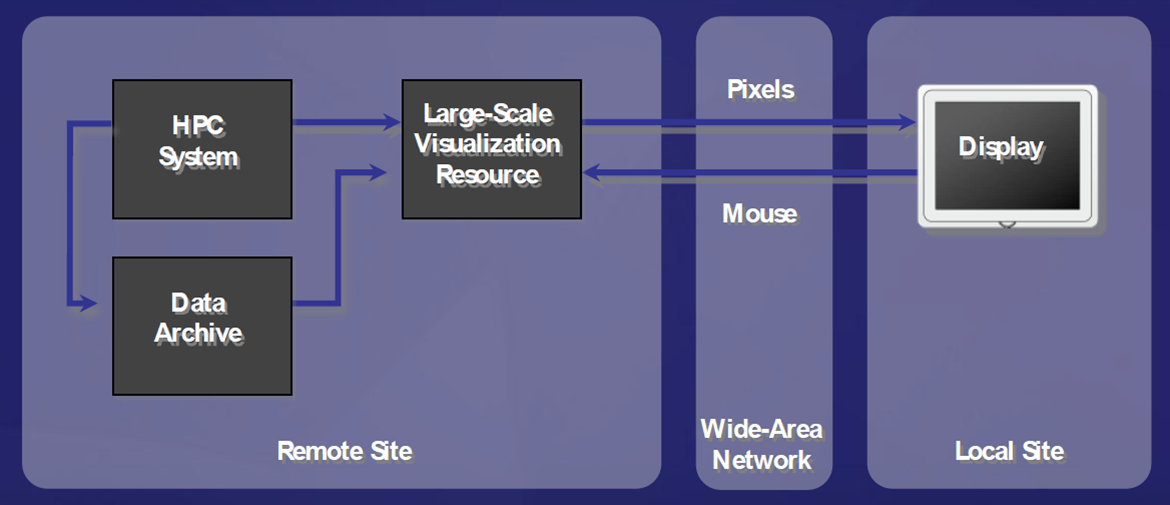
\includegraphics{\picdir/RemoteVis}}

GPU enables Operating room portable compute technology.
\end{frame}

%%%%%%%%%%%%%%%%%%%%%%%%%%%%%%%%%%%%%%%%%%%%%%%%%%%%%%%%%%%%%%%%%%%%%%%%%%%%
\frame{ \frametitle{Treatment Workflow: Planning, Monitoring, \& Control}

\begin{itemize}
\item  \alert{Multiple timescales of interaction} between imaging
        feedback and predictive simulation
  \begin{itemize}
   \item  \alert{Prospective 3D Treatment Planning}
   \item  \alert{Model Prediction Assisted Monitoring}
   \item  \alert{Stochastic Optimal Control}
  \end{itemize}
\end{itemize}
\scalebox{0.17}{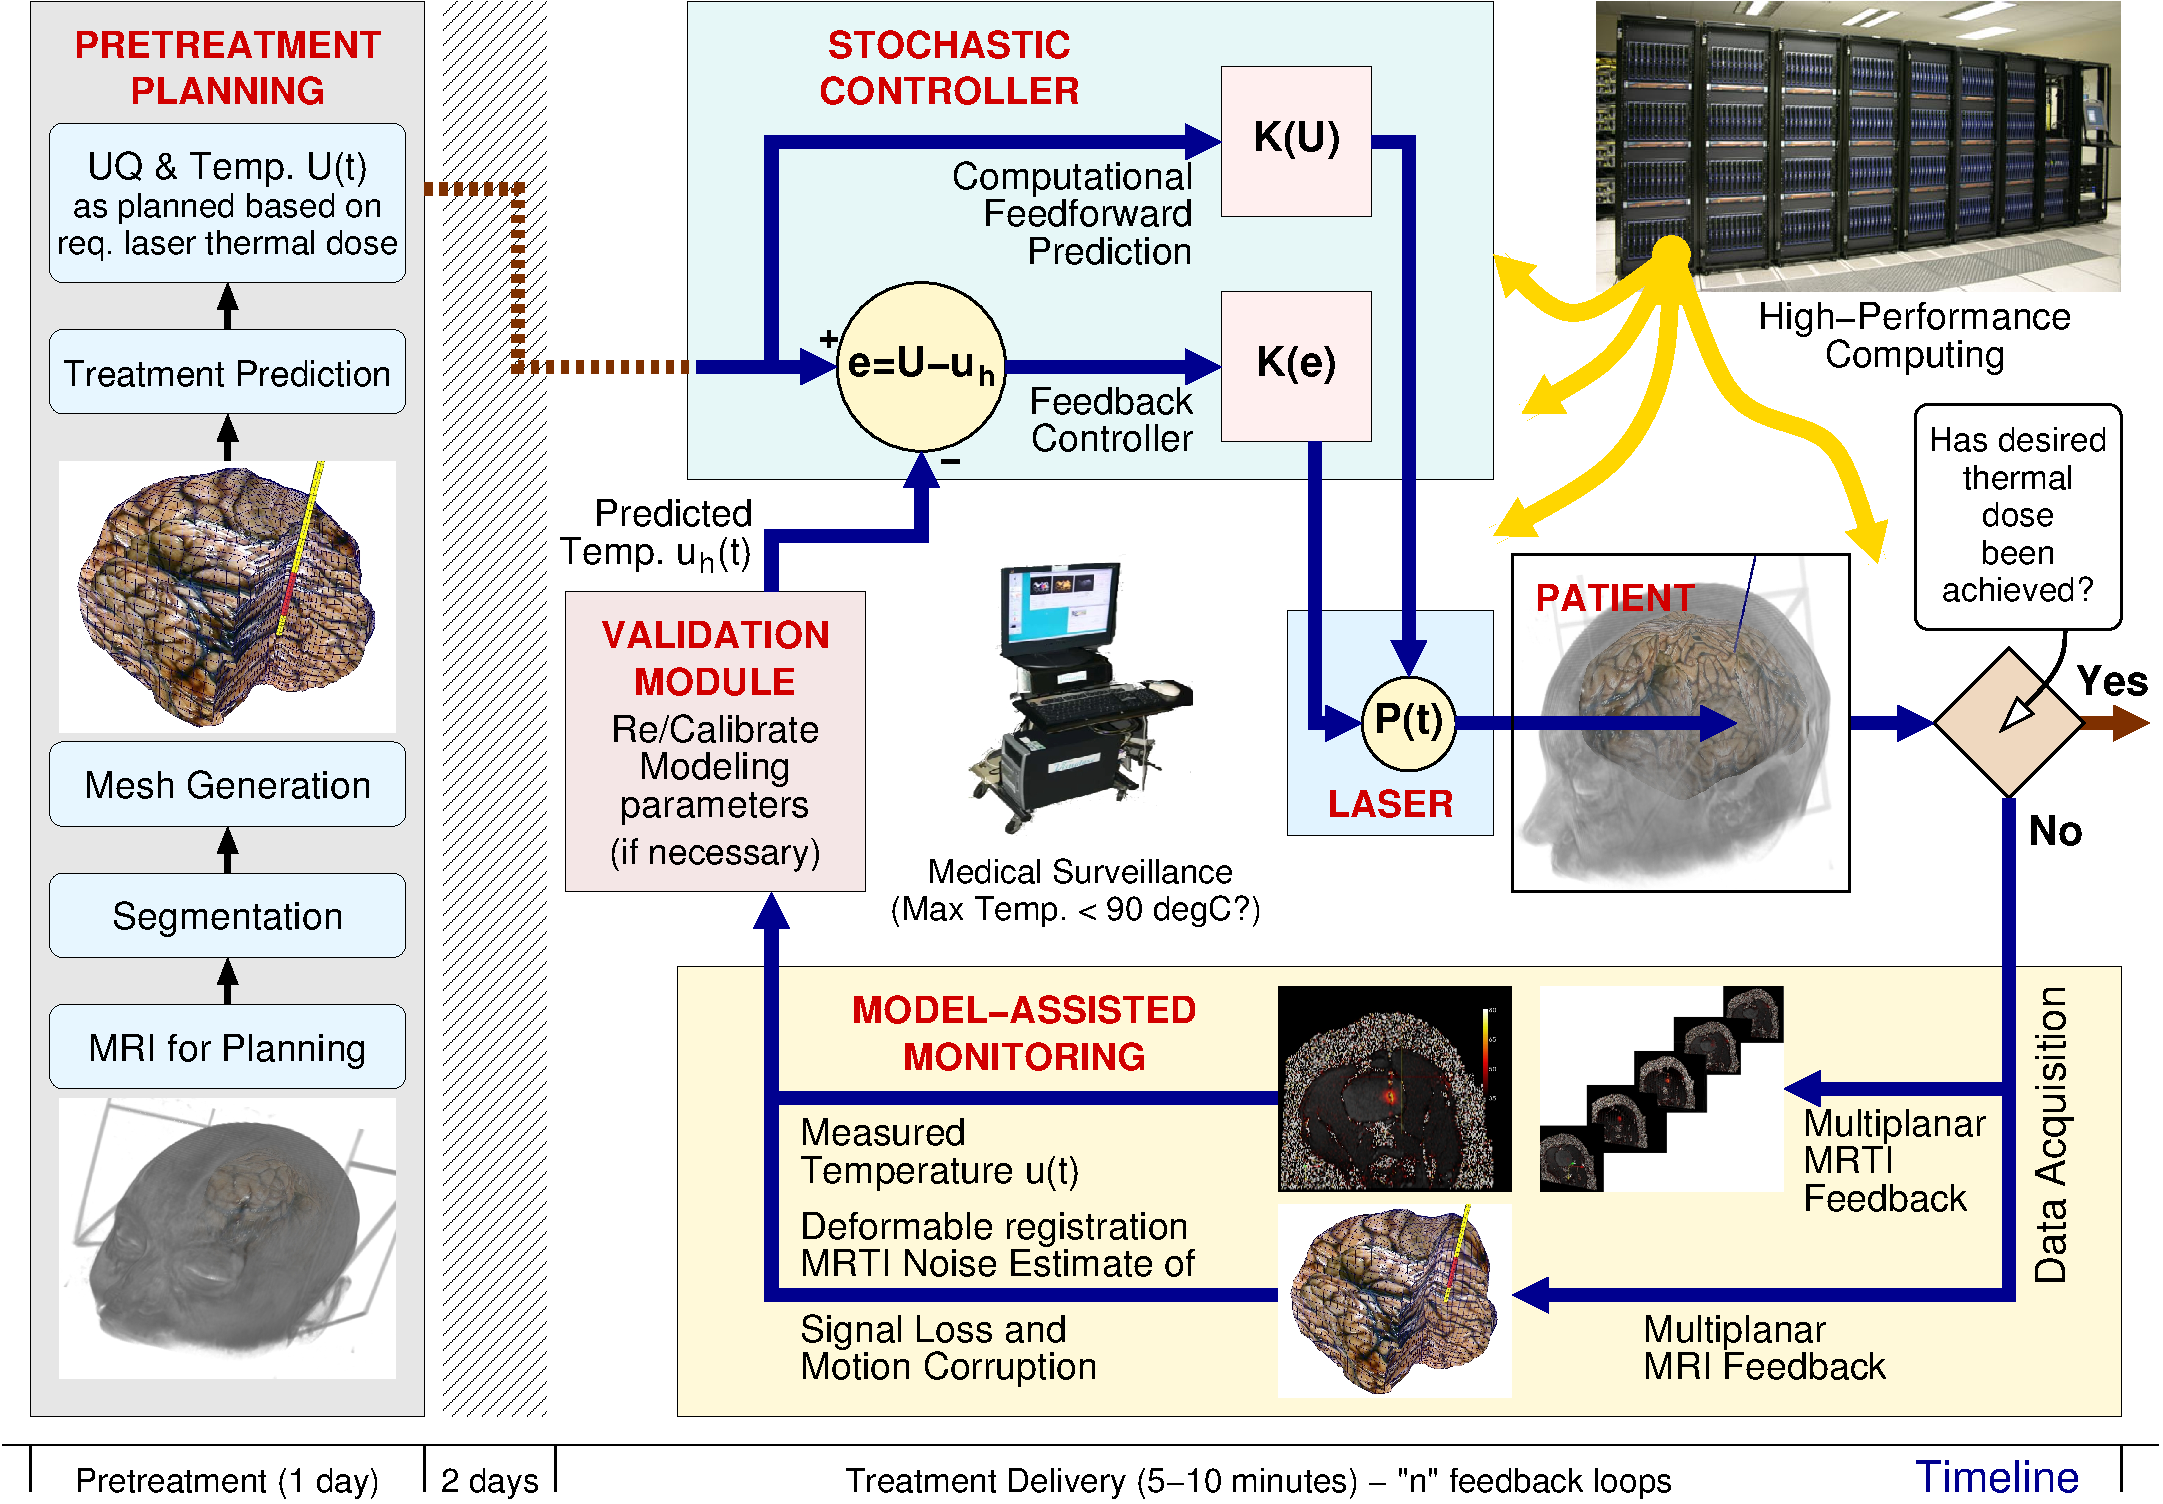
\includegraphics{\picdir/TreatmentSystem}}
}
%%%%%%%%%%%%%%%%%%%%%%%%%%%%%%%%%%%%%%%%%%%%%%%%%%%%%%%%%%%%%%%%%%%%%%%%%%%%
\frame{ \frametitle{libMesh}
\begin{itemize}
  \item Abstract C++ parallel computing framework for FEM
  \item Builds on top of PETSC and other high quality packages
  \item \htmladdnormallink{http://libmesh.sourceforge.net/}
                          {http://libmesh.sourceforge.net/}
  \item \htmladdnormallink{Documentation}
  {http://libmesh.sourceforge.net/examples.php}
  provides working example problems to get started
   \begin{itemize}
     \item  complexity built in a hierarchy from 1d diffusion problems
to 3d Navier Stokes
   \end{itemize}
\end{itemize}
}
%%%%%%%%%%%%%%%%%%%%%%%%%%%%%%%%%%%%%%%%%%%%%%%%%%%%%%%%%%%%%%%%%%%%%%%%%%%
\frame{ \frametitle{libMesh: Abstract Assembly}
\begin{itemize}
  \item Assembly of abstract variational problem using the 
  \htmladdnormallink{Poisson} {http://libmesh.sourceforge.net/ex4.php}
($\Delta u = f$) problem as an example.
\[ \begin{split}
 \text{Find } u  & \in \mathcal{V}: \\
   &  B(u,v) = F(v) \qquad \forall v \in \mathcal V
\end{split} \]
  \item Galerkin Expansion $v = v_i e_i$, $u = u_j e_j$
\[
       \begin{bmatrix}
 . &            & . \\
   & B(e_j,e_i) &   \\
 . &            & . \\
        \end{bmatrix}
       \begin{bmatrix}
        . \\
       u_j          \\
        . \\
        \end{bmatrix}
=
  \begin{bmatrix}
    . \\
  F(e_i)    \\
    . \\
  \end{bmatrix}
\]
\end{itemize}
}
%%%%%%%%%%%%%%%%%%%%%%%%%%%%%%%%%%%%%%%%%%%%%%%%%%%%%%%%%%%%%%%%%%%%%%%%%%%
\begin{frame}[fragile]
\frametitle{libMesh: Abstract Assembly}
\begin{semiverbatim}
\scriptsize
// setup iterators
MeshBase::const_element_iterator    
          el     = mesh.local_elements_begin();
for ( ; el != mesh.local_elements_end(); ++el) // loop over elements
 \{
  //loop over quadrature points
  for (unsigned int qp=0; qp<qrule.n_points(); qp++)
   //loop over shape functions
   for (unsigned int i=0; i<phi.size(); i++)
     for (unsigned int j=0; j<phi.size(); j++)
       B(i,j) += JxW[qp]*(dphi[i][qp]*dphi[j][qp]);

  //loop over quadrature
  for (unsigned int qp=0; qp<qrule.n_points(); qp++)
    //loop over shape functions
    for (unsigned int i=0; i<phi.size(); i++) 
       F(i) += JxW[qp]*f[qp]*phi[i][qp];
 \}
\end{semiverbatim}
\end{frame}

%%%%%%%%%%%%%%%%%%%%%%%%%%%%%%%%%%%%%%%%%%%%%%%%%%%%%%%%%%%%%%%%%%%%%%%%%%%
\begin{frame}[fragile]
\frametitle{libMesh: Abstract Assembly}
\begin{semiverbatim}
\scriptsize
// Define the system
LinearImplicitSystem& system =
  equation_systems.add_system<LinearImplicitSystem> ("Poisson");
// get dof map
const DofMap& dof_map = system.get_dof_map();
// loop over elements
for ( ; el != mesh.local_elements_end(); ++el) 
 \{
      dof_map.dof_indices (elem, dof_indices);
           .
           /*Assembly*/
           .
      system.matrix->add_matrix (B, dof_indices);
      system.rhs->add_vector    (F, dof_indices);
 \}
// matrix solve
system.solve()
\end{semiverbatim}
\end{frame}

%%%%%%%%%%%%%%%%%%%%%%%%%%%%%%%%%%%%%%%%%%%%%%%%%%%%%%%%%%%%%%%%%%%%%%%%%%%
\begin{frame}
\scalebox{0.36}{ 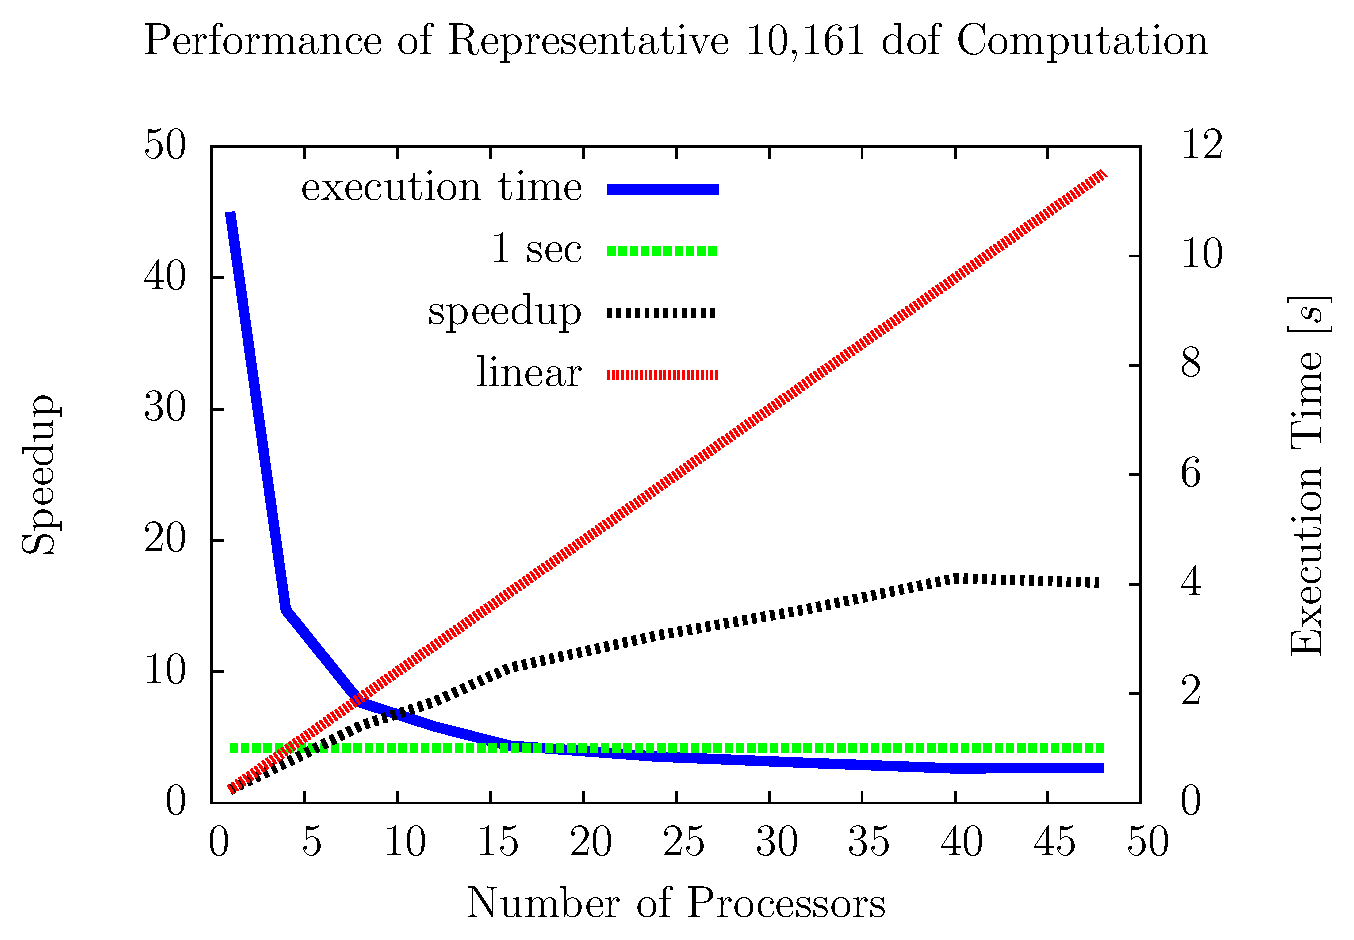
\includegraphics{\picdir/performance} }
{\tiny Shown is the speedup as a function of processors
and execution time for a representative 10 second simulation (10 nonlinear
state solve combined with 10 linear adjoint solve on 10000 dof system)
The fastest execution time is of the highest priority,
the efficiency of the computation is sacrificed for execution time.
} 
\end{frame}

%%%%%%%%%%%%%%%%%%%%%%%%%%%%%%%%%%%%%%%%%%%%%%%%%%%%%%%%%%%%%%%%%%%%%%%%%%%
\frame{ \frametitle{Introduction}
\framesubtitle{
MR guided Laser Induced Thermal Therapies (MRgLITT)
}

\begin{minipage}{.48\textwidth}
\scalebox{0.34}{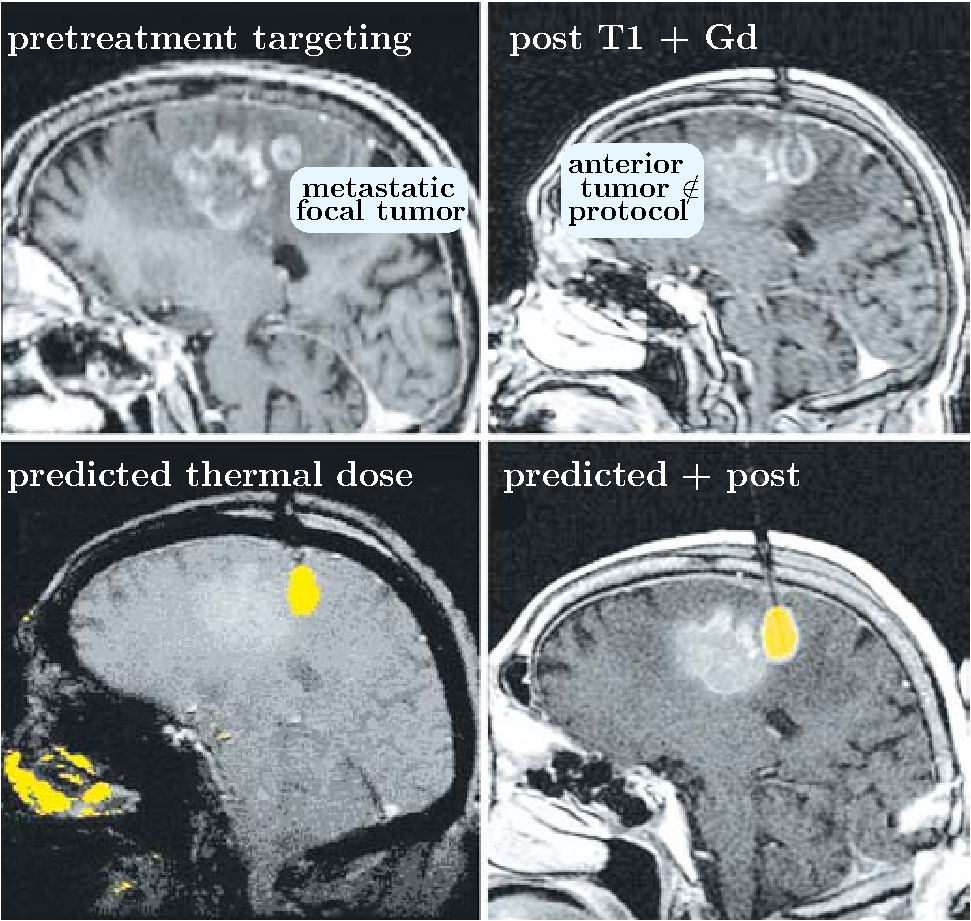
\includegraphics{\picdir/prepostMRgLITT}}
\rule{2.0in}{0.3mm}\\
\tiny
\hspace{.04in} A.~Carpentier, \textit{Neurosurgery} 63:1 (2008)
\vspace{-.1in}
%AB OBJECTIVE: We report the initial results of a pilot clinical trial exploring
%the safety and feasibility of the first real-time magnetic resonance-guided
%laser-induced thermal therapy of treatment-resistant focal metastatic
%intracranial tumors. METHODS: Patients with resistant metastatic intracranial
%tumors who had previously undergone chemotherapy, whole-brain radiation
%therapy, and radiosurgery and who were recused from surgery were eligible for
%this trial. Under local anesthesia, a Leksell stereotactic head frame was used
%to insert a water-cooled interstitial fiberoptic laser applicator inside the
%cranium. In the bore of a magnetic resonance imaging (MRI) scanner, laser
%energy was delivered to heat the tumor while continuous MRI was performed. A
%computer workstation extracted temperature-sensitive information to display
%images of laser heating and computed estimates of the thermal damage zone.
%Posttreatment MRI scans were used to confirm the zone of thermal necrosis, and
%follow-up was performed at 7, 15, 30, and 90 days after treatment. RESULTS: In
%all cases, the procedure was well tolerated without secondary effect, and
%patients were discharged to home within 14 hours after the procedure. Follow-up
%imaging showed an acute increase in apparent lesion volume followed by a
%gradual and steady decrease. No tumor recurrence within thermal ablation zones
%was noted. CONCLUSION: In this ongoing trial, a total of four patients have had
%six metastatic tumors treated with laser thermal ablations. Magnetic
%resonance-guided laser-induced thermal therapy appears to provide a new,
%efficient treatment for recurrent focal metastatic brain disease. This therapy
%is a prelude to the future development of closed-head interventional MRI
%techniques in neurosurgery. Copyright (C) by the Congress of Neurological
%Surgeons
\end{minipage}~\begin{minipage}{.51\textwidth}
\small
\begin{itemize}
%\item  Image guidance facilitates
%       treatment planning, targeting, %localizing,
%       monitoring, verification
%  \begin{itemize}
%   \item  increase safety and efficacy and facilitates minimally invasive
%          therapies previously not possible/safe
%   \item  MR images are used to navigate the applicator to the target
%volume and monitor the heating to
%         avoid damaging critical structures with applicator
%  \end{itemize}
\item  MRgLITT
a minimally invasive alternative to
conventional surgery and SRS
\item Actively cooled diffusing interstitial laser fiber
under thermal image monitoring
%MRTI monitoring in those organs are all we've done in vivo.
\item Focal lesions in brain, prostate, liver, bone
   \begin{itemize} \scriptsize
     \item \alert{MR to plan, target, monitor, and post treatment
verification}
   \end{itemize}
%One idea you might want to interleave in there is "dose" and the fact
%that damage is cumulative and a major goal is outcome prediction based
%on cumulative exposure.
\item \alert {Major goal:} Thermal dose (10-15W,30-180s)
      used as immediate verification  of delivery
   \begin{itemize} \scriptsize
      \item $<$3cm diameter, can pull back fiber
   \end{itemize}
\end{itemize}
\end{minipage}
}
%%%%%%%%%%%%%%%%%%%%%%%%%%%%%%%%%%%%%%%%%%%%%%%%%%%%%%%%%%%%%%%%%%%%%%%%%%%
\begin{frame}
\frametitle{Laser}

10mm axial length \\
\scalebox{0.65}{ 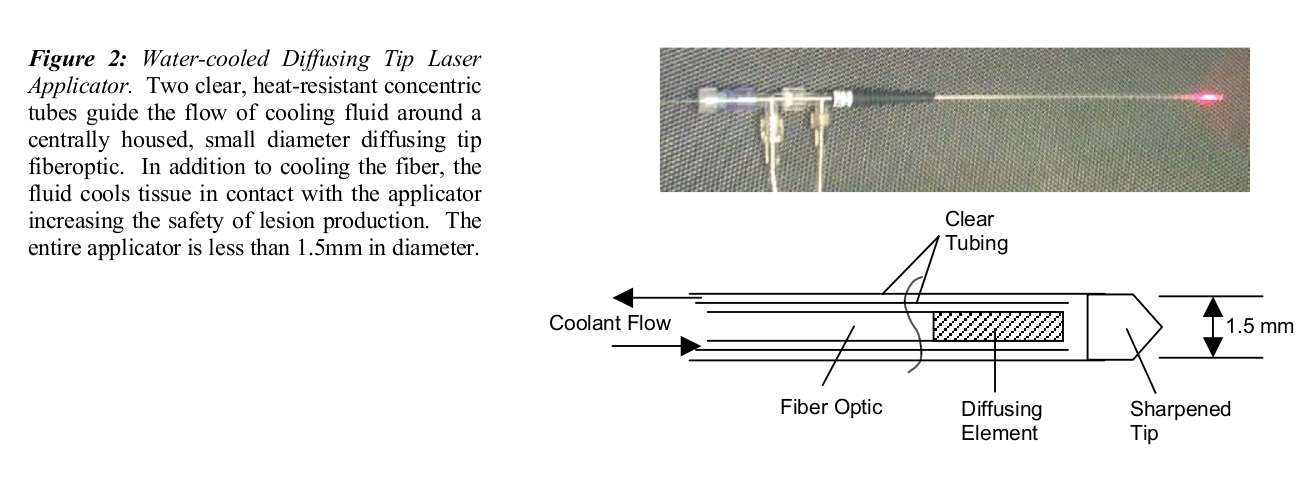
\includegraphics{\picdir/cooledtip}}

\end{frame}

%%%%%%%%%%%%%%%%%%%%%%%%%%%%%%%%%%%%%%%%%%%%%%%%%%%%%%%%%%%%%%%%%%%%%%%%%%%
\frame{ \frametitle{Bioheat Transfer Model}
\begin{minipage}{.47\linewidth}
\hspace{-.4in}
\scalebox{0.26}{ 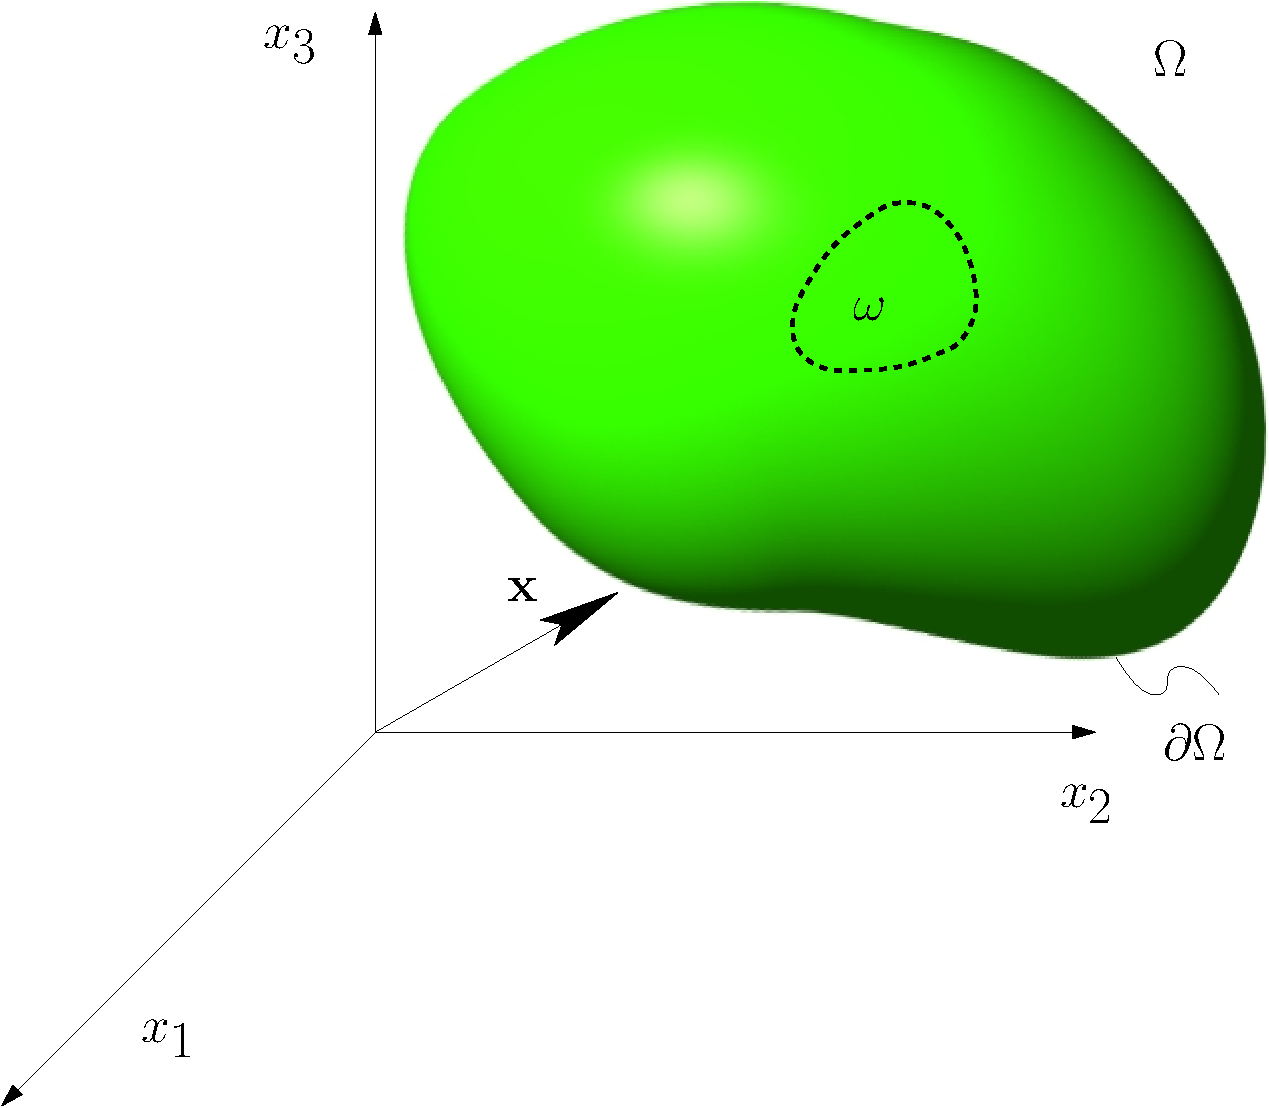
\includegraphics{\picdir/idealmodel}}
\end{minipage}~\begin{minipage}{.52\linewidth}
\footnotesize
\begin{itemize}
  \item no mass flux across boundary, $\partial \Omega$
  \item no motion, deformation, or applied forces
  \item muscle, fat blood, etc. is represented as a single continuous medium
           that may have spatially varying properties.
  \item the presence of the blood within the tissue acts as a
volumetric heating term at every point within the body $\Omega$
  \item laser source modeled as spherically symmetric isotropic soln
        of light/tissue transport eqn
\end{itemize}
\end{minipage}

\rule{2.0in}{0.3mm}\\
\alert{
\scriptsize
\hspace{.04in} H.H.~Pennes, J. App. Physiology. (1948).
  \\
\hspace{.04in} A.J.~Welch, Optical-Thermal Response
\\
\hspace{.64in}              of Laser-Irradiated Tissue.  (1995).

}
}
%
%%%%%%%%%%%%%%%%%%%%%%%%%%%%%%%%%%%%%%%%%%%%%%%%%%%%%%%%%%%%%%%%%%%%%%%%%%%
\frame{ \frametitle{Bioheat Transfer Model}

 \footnotesize
\begin{boxedminipage}{\linewidth}
{\color{blue}\underline{The Non-Linear Pennes Model}}
\[
 \underbrace{
 \rho  c_p \frac{\partial u}{\partial t}
 -\nabla \cdot ( \alert{k(u,\textbf{x},\beta)} \nabla u)
 }_\text{Standard}
 +\underbrace{ \alert{\omega(u,\textbf{x},\beta)} c_{blood} (u - u_a )}_\text{Empirical}
 = Q_{laser}(\beta,\textbf{x},t) \quad \text{in } \Omega
 \]
  \[ - \alert{k(u,\textbf{x},\beta)} \nabla u \cdot \textbf{n} = h (u - u_{\infty})
        \qquad \text{on } \partial \Omega_C
\]\[
   - \alert{k(u,\textbf{x},\beta)} \nabla u \cdot \textbf{n} = \mathcal{G}
        \qquad \text{on } \partial \Omega_N
  \]
 \[
   u(\textbf{x},0) = u^0 \qquad \text{in } \Omega
 \]
\end{boxedminipage}


\vspace{.2in}

\begin{tabular}{ll}
$\rho$ density $[\frac{kg}{m^3}]$ &
$k(u,\textbf{x},\beta)$ thermal conductivity $[\frac{W}{m\cdot K}]$ \\
$\omega(u,\textbf{x},\beta)$ blood perfusion $[\frac{kg}{s \cdot m^3}]$ &
 $P(t)$ Power $[W]$ \\
$c_p$ specific heat $[\frac{J}{kg \cdot K}]$ &
 $\mu_a$, $\mu_s$ coeff. of absorb/scattering $[\frac{1}{m}]$ \\
 $g$ anisotropy factor&
 $\textbf{x}_0$  laser position $[m]$ \\
\end{tabular}

}
%%%%%%%%%%%%%%%%%%%%%%%%%%%%%%%%%%%%%%%%%%%%%%%%%%%%%%%%%%%%%%%%%%%%%%%%%%%
\frame{ \frametitle{Laser Model}
Consider Pennes model coupled to a diffusion theory model of light
transport in tissue. The total fluence at a point is given by the
sum of the scattered and primary light $\varphi_t(x,t) = z(x,t) + E(x,t)$.
}

%%%%%%%%%%%%%%%%%%%%%%%%%%%%%%%%%%%%%%%%%%%%%%%%%%%%%%%%%%%%%%%%%%%%%%%%%%%
\frame{ \frametitle{Laser Model}
Through the diffusion model,
the scattered fluence $z$ is obtained from the 
known irradiance $E(x,t)$ (primary source of photons) 
and its flux $\textbf{F}(x,t)$.
{\small
\[
\nabla \cdot \left( \frac{1}{3 \mu_{tr} } \nabla \varphi_d(\mathbf{r}) \right)
 - \mu_a \varphi_d(\mathbf{r}) 
= 
- \mu_s^*  E(\mathbf{r})
+   \nabla \cdot \left( \frac{g^* \mu_s^*}{\mu_{tr}} E(\mathbf{r}) \hat{s}_0 \right)
\]
\[
 \frac{1}{c(x)}
 \frac{\partial(z+E)}{\partial t}
 -{\color{red}\mu_a(\textbf{x})} z 
 +{\color{red}\mu_s^*(\textbf{x},m)} E
 = \nabla \cdot 
   \left( 
   - \frac{ \nabla z }{3\mu_{tr}(\textbf{x},m)} 
   + \frac{ {\color{red}\mu_s^*}(\textbf{x},m) g^* }{3\mu_{tr}(\textbf{x},m)}
       \textbf{F}
   \right)
\qquad
  \mu_{tr}(\textbf{x},m)  = 
                 {\color{red}\mu_a(\textbf{x},m)} + 
                    {\color{red}\mu_s(\textbf{x},m)} (1-g)
\]
}
}
%%%%%%%%%%%%%%%%%%%%%%%%%%%%%%%%%%%%%%%%%%%%%%%%%%%%%%%%%%%%%%%%%%%%%%%%%%%
\frame{ \frametitle{Laser Model}
The irradiance is provided by a photon flux emitted throughout
the domain of an interstitial laser fiber $\Omega_{tip}$.
The photons are emittied by an applied power density,
$P^* \left[\frac{W}{m^3}\right]$. Each position in the domain $\hat{x}$
is treated as a point source of irradiance
\[
dE(x,\hat{x})= 
             \frac{P^*(t)d\hat{x}}{4\pi \|\textbf{x} -
\hat{\textbf{x}}\|^2}
\]
}
%%%%%%%%%%%%%%%%%%%%%%%%%%%%%%%%%%%%%%%%%%%%%%%%%%%%%%%%%%%%%%%%%%%%%%%%%%%
\frame{ \frametitle{Laser Model}
The total irradiance and flux is the integral of each attenuated point source.
\[
\begin{split}
E(x,t) & = \int_{\Omega_{tip}} 
             \frac{P^*(t)}{4\pi \|\textbf{x} - \hat{\textbf{x}}\|^2}
             \exp\left(\mu_t^*(\textbf{x},m)
                         \|\textbf{x} - \hat{\textbf{x}}\|\right) d\hat{x}
 \\
\textbf{F}(x,t) & = \int_{\Omega_{tip}} 
             \frac{P^*(t)}{4\pi \|\textbf{x} - \hat{\textbf{x}}\|^2}
             \exp\left(\mu_t^*(\textbf{x},m) 
                         \|\textbf{x} - \hat{\textbf{x}}\|\right) 
\frac{\textbf{x} - \hat{\textbf{x}} }{ \|\textbf{x} - \hat{\textbf{x}}\| }
d\hat{x}
\end{split} 
\]
\[
  \mu_t^*(\textbf{x},m)  = 
                 {\color{red}\mu_a(\textbf{x},m)} + 
                    {\color{red}\mu_s(\textbf{x},m)}  
\]
}
%%%%%%%%%%%%%%%%%%%%%%%%%%%%%%%%%%%%%%%%%%%%%%%%%%%%%%%%%%%%%%%%%%%%%%%%%%%
\frame{ \frametitle{Laser Model}
\textbf{${\color{red}\mu_t(\textbf{x},m)}$ should be the average over
the path length for the heterogenious case}.
An analytic solution may be obtained by approximating the integral for
the irradiance and flux as
{\small
\[
\begin{split}
E(x,t) 
  & \approx 
  \sum_{e\in \Omega_{tip}} E_e(x,t)
  =
  \sum_{e\in \Omega_{tip}} 
          \frac{\Delta V_e P^*(t)}{4\pi \|\textbf{x} - \hat{\textbf{x}}_e\|^2}
          \exp\left(\mu_t^*(\textbf{x},m) 
                 \|\textbf{x} - \hat{\textbf{x}}_e\|\right) 
 \\
\textbf{F}(x,t) 
  & \approx 
    \sum_{e\in \Omega_{tip}} \textbf{F}_e(x,t) 
  = \sum_{e\in \Omega_{tip}} 
          \frac{\Delta V_e P^*(t)}{4\pi \|\textbf{x} - \hat{\textbf{x}}\|^2}
          \exp\left(\mu_t^*(\textbf{x},m) 
                         \|\textbf{x} - \hat{\textbf{x}}\|\right) 
\frac{\textbf{x} - \hat{\textbf{x}} }{ \|\textbf{x} - \hat{\textbf{x}}\| }
\end{split} 
\]
}
where $\Delta V_e$ is the volume and 
$\hat{\textbf{x}}_e$ is the centroid.
}

%%%%%%%%%%%%%%%%%%%%%%%%%%%%%%%%%%%%%%%%%%%%%%%%%%%%%%%%%%%%%%%%%%%%%%%%%%%
\frame{ \frametitle{Laser Model}
By linearity, each element in the discretization may be treated as
an uncoupled and independent source in the light diffusion equation.
\[
\begin{split}
 -{\color{red}\mu_a(\textbf{x})} z_e 
 +{\color{red}\mu_s^*(\textbf{x},m)} E_e
 = \nabla \cdot 
  &\left( 
   - \frac{ \nabla z_e }{3\mu_{tr}(\textbf{x},m)} 
   + \frac{ {\color{red}\mu_s^*}(\textbf{x},m) g^* }{3\mu_{tr}(\textbf{x},m)} 
       (\textbf{F})_e
   \right)  
   \\  
  & \qquad \forall e \in \Omega_{tip}
\end{split}
\]
The fluence resulting from each element source $(\varphi_t)_e$
may be obtained from the classical isotropic point source
solution \cite{Welch95}.
}
%%%%%%%%%%%%%%%%%%%%%%%%%%%%%%%%%%%%%%%%%%%%%%%%%%%%%%%%%%%%%%%%%%%%%%%%%%%
\frame{ \frametitle{Laser Model}
The total emanating fluence is the superposition of the element wise
solutions and reduces to a volume weighted sum over the elements.
\[
\begin{split}
   \varphi_t
 &  = \sum_{e \in \Omega_{tip}}
 {\color{red}P^*(t)}  V_e  \left(
   \frac{3\mu_{tr} \exp(-\mu_{eff} \|\textbf{x} -{\color{red}\textbf{x}_e}\|) }
      {4\pi \|\textbf{x}-{\color{red}\textbf{x}_e}\|}
 - 
      \frac{ 
             \exp(-\mu_t^* \|\textbf{x} -{\color{red}\textbf{x}_e}\|) }
           {2\pi \|\textbf{x}-{\color{red}\textbf{x}_e}\|^2}
   \right)
 \\
 & \approx
    \sum_{e \in \Omega_{tip}}
 {\color{red}P^*(t)}  V_e 
   \frac{3\mu_{tr} \exp(-\mu_{eff} \|\textbf{x} -{\color{red}\textbf{x}_e}\|) }
      {4\pi \|\textbf{x}-{\color{red}\textbf{x}_e}\|}
\end{split}
\]
\[
Q_{laser}(\beta,\textbf{x},t)   = \alert{\mu_a} \varphi_t
\hspace{-1.0in}
\begin{split}
  \mu_{tr} &  = \alert{\mu_a } +  \alert{\mu_s} (1-g) \qquad
\\
  \mu_{eff} & = \sqrt{3 \alert{\mu_a} \mu_{tr}}
\end{split} \]


}

\end{document}
